\subsection*{Baseline por desbalance}
El dataset presenta alto desbalance (baja recompra). Por ello, se reportó un baseline trivial que predice churn para todos: logra accuracy alta pero F1 para no-churn es 0. Esto justifica el uso de métricas enfocadas a la clase minoritaria.

\subsection*{Modelos}
Se compararon:
\begin{itemize}
  \item \textbf{Regresión logística} (con \texttt{class\_weight=balanced}), variando $C$ y el umbral de decisión.
  \item \textbf{Random Forest} (con \texttt{class\_weight=balanced\_subsample}), con variantes de \texttt{max\_depth} y \texttt{min\_samples\_leaf}.
\end{itemize}

\subsection*{Métricas}
Además de accuracy, se reportaron métricas relevantes para no-churn (recompra): \texttt{pr\_auc\_nochurn\_0} y \texttt{f1\_nochurn\_0}, junto con matrices de confusión y curvas Precision--Recall para la clase no-churn.

\subsection*{Selección de umbral}
Se optimizó el umbral para maximizar \texttt{f1\_nochurn\_0}. En los experimentos se obtuvo un umbral operativo de 0.12.

\noindent \textbf{Run ganador (MLflow).} Se seleccionó el run \texttt{logreg\_C0.1\_thr012} por obtener el mejor valor de \texttt{pr\_auc\_nochurn\_0} (y un alto \texttt{f1\_nochurn\_0}) en la comparación de runs.



\begin{figure}[H]
\centering
\begin{subfigure}[b]{0.48\textwidth}
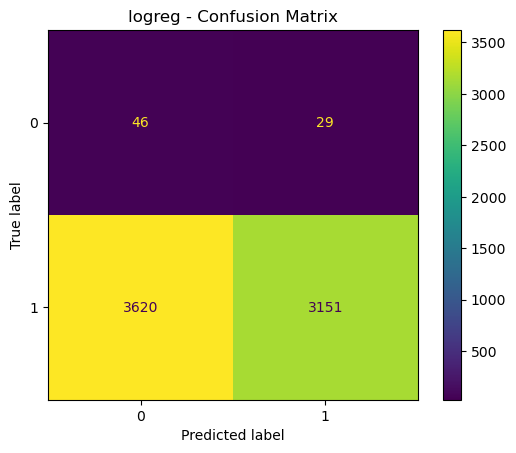
\includegraphics[width=\textwidth]{evidence/model/FIG_MODEL_01_cm_logreg.png}
\caption{Matriz de confusión (LogReg).}
\end{subfigure}\hfill
\begin{subfigure}[b]{0.48\textwidth}
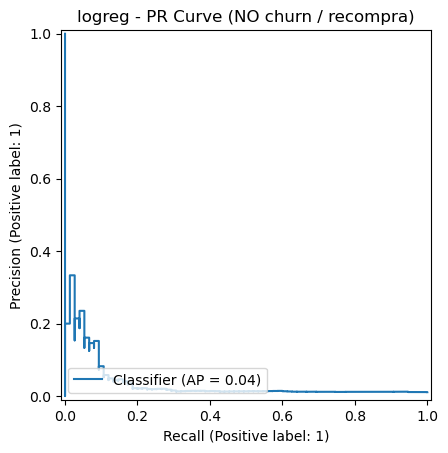
\includegraphics[width=\textwidth]{evidence/model/FIG_MODEL_02_pr_logreg.png}
\caption{Curva PR para no-churn (LogReg).}
\end{subfigure}
\caption{Evaluación del modelo.}
\end{figure}